\subsection{Metodologia}
\begin{frame}
    \frametitle{Metodologia}
    \framesubtitle{Base de \'Audio Transcrita}
    \begin{center}
        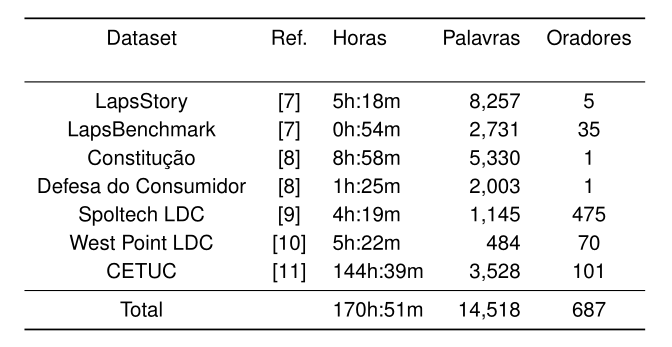
\includegraphics[width=0.8\textwidth]{Figures/db}
    \end{center}
\end{frame}

\begin{frame}
    \frametitle{Metodologia}
    \framesubtitle{Treinamento dos AMs}
    \begin{center}
        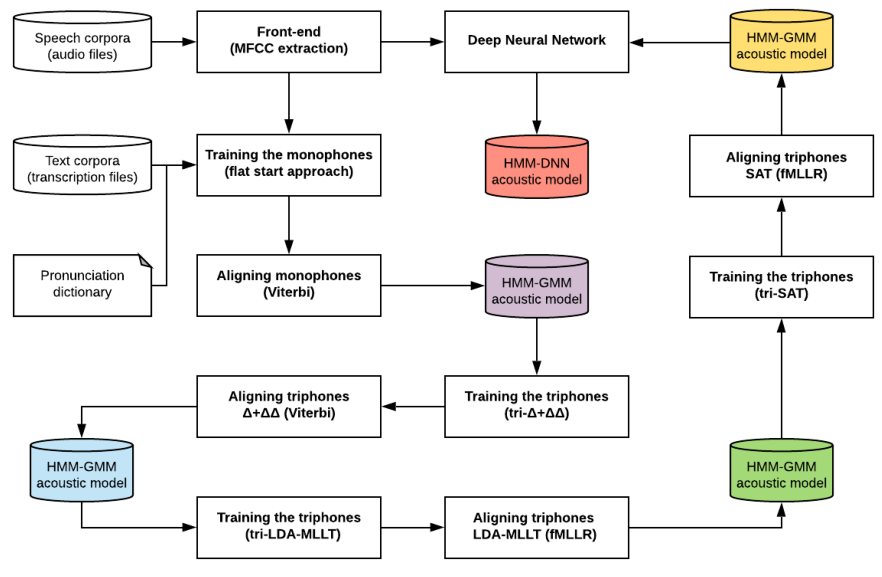
\includegraphics[width=0.8\textwidth]{Figures/training}
    \end{center}
\end{frame}

\begin{frame}
    \frametitle{Testes}
    \begin{itemize}
        \item \textit{Dataset} de Avalia\c c\~ao
        \begin{itemize}
            \item 200 enunciados falados por um orador masculino
            \item Total de 7min58s de \'audio alinhado manualmente
        \end{itemize}
        \item Caracter\'istica comparada: limite fon\'etico
        \begin{itemize}
            \item Diferen\c ca entre o tempo final da ocorrência do fonema em ambos alinhamentos, pelo alinhador e alinhado manualmente
        \end{itemize}
    \end{itemize}
\end{frame}
